\begin{savequote}[45mm]
\ascii{Any fool can write code that a computer can understand. Good programmers write code that humans can understand.}
\qauthor{\ascii{- Martin Flower}}
\end{savequote}

\chapter{原理与概念} 
\label{ch:bazel-concept}

\section{概念}

\begin{content}

\subsection{领域模型}

\begin{figure}[H]
\centering
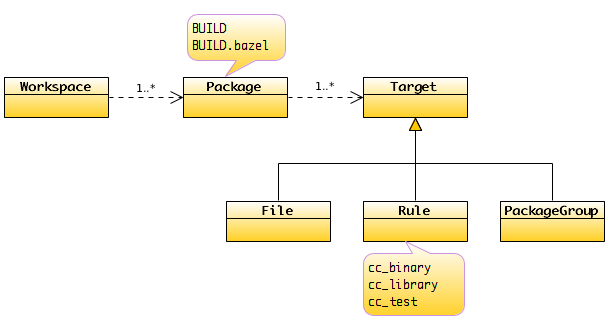
\includegraphics[width=0.8\textwidth]{figures/bazel-domain-model.png}
\caption{领域模型} 
 \label{fig:bazel-domain-model}
\end{figure}

\subsection{工作区}

一般地,在项目的根目录创建一个\ascii{WORKSPACE}文件,它表示的该项目的\emph{工作区}(\ascii{Workspace})。项目中的所有的文件,包括待构建的源文件、构建输出的目标文件,及其外部依赖都归属于该\emph{工作区}。\ascii{WORKSPACE}文件用于声明项目的外部依赖;如果项目不存在外部依赖,\ascii{WORKSPACE}的内容可为空。

工作区为项目的构建提供了一个安全的隔离环境。例如,你在本地正在构建两个\cpp{}项目,它们都依赖了\ascii{protobuf};不幸的是,它们依赖了不同版本的\ascii{protobuf}。此时问题变得相当棘手,\ascii{/usr/local/include}目录到底放哪个版本呢?

归功于\ascii{Bazel}良好的隔离性,每个项目的工作区都是独立的,它们将依赖控制在各自的工作区,从而避免了第三方库的名字冲突。

\subsection{包}

含有\ascii{BUILD}或\ascii{BUILD.bazel}的目录,\ascii{Bazel}称之为\emph{包}(\ascii{Package})。在一个包中,可以包含该目录,及子目录的所有文件(包含\ascii{BUILD}的子包除外)。需要关注的是,子包独立于父包,父包不包括子包的内容。

\subsection{目标}

在\ascii{BUILD}文件中,可以定义零个或多个\emph{目标}(\ascii{Target})。一般地,目标包括\emph{文件}(\ascii{File}),\emph{规则}(\ascii{Rule}),\emph{包集合}(\ascii{Package Group})三种基本类型。

文件包括源文件和派生文件。例如,程序员实现的\cpp{}头文件和实现文件称为源文件,而由\ascii{protoc}机器生成的头文件和实现文件则称为派生文件。

规则由输入、输出、动作三元祖构成,通过规则之间的依赖关系,构建了\ascii{DAG}图。依赖关系具有多种形式,而且与语言相关。例如,在编译时,\ascii{A}依赖于\ascii{B}的头文件;在链接时,\ascii{A}依赖于\ascii{B}的符号;在运行时,\ascii{A}依赖于\ascii{B}的数据。

包集合较为特殊,它标识一组包。它由\ascii{package\_group}定义。使用包集合,可以很方便地某一个规则的可见性一并分配给该集合中的所有包。

\subsubsection{命名}


\subsubsection{规则}



\end{content}
